% Hlavicka pro protokoly z fyzikalniho praktika.
% Verze pro: LaTeX
% Verze hlavicky: 22. 2. 2007
% Autor: Ustav fyziky kondenzovanych latek
% Ke stazeni: www.physics.muni.cz/ufkl/Vyuka/
% Licence: volne k pouziti, nejlepe k vcasnemu odevzdani protokolu z Vaseho mereni.


\documentclass[czech,11pt,a4paper]{article}
\usepackage[T1]{fontenc}
\usepackage{graphicx, animate}
\usepackage{mathtools}
\usepackage{amssymb}
\usepackage{amsthm}
\usepackage{thmtools}
\usepackage{xcolor}
\usepackage{nameref}
\usepackage{babel}
\usepackage{hyperref}
\usepackage{multicol}
\usepackage[export]{adjustbox}
\usepackage{subcaption}
\usepackage{caption}
\usepackage{multirow}
\usepackage{float}
\usepackage{placeins}
\usepackage{biblatex}
\graphicspath{ {./images/} }




%%% Nemente:
\usepackage[margin=2cm]{geometry}
\newtoks\jmenopraktika \newtoks\jmeno \newtoks\datum
\newtoks\obor \newtoks\skupina \newtoks\rocnik \newtoks\semestr
\newtoks\cisloulohy \newtoks\jmenoulohy
\newtoks\tlak \newtoks\teplota \newtoks\vlhkost
%%% Nemente - konec.


%%%%%%%%%%% Doplnte pozadovane polozky:

\jmenopraktika={Fyzikální praktikum 2}  % nahradte jmenem vaseho predmetu
\jmeno={Teodor Duraković}            % nahradte jmenem mericiho
\datum={2.~prosince 2024}        % nahradte datem mereni ulohy
\obor={F}                     % nahradte zkratkou vami studovaneho oboru
\skupina={Po 14:00}            % nahradte dobou vyuky vasi seminarni skupiny
\rocnik={II}                  % nahradte rocnikem, ve kterem studujete
\semestr={III}                 % nahradte semestrem, ve kterem studujete

\cisloulohy={9}               % nahradte cislem merene ulohy
\jmenoulohy={Závislost indexu lomu skla na vlnové délce} % nahradte jmenem merene ulohy

\tlak={994}                   % nahradte tlakem pri mereni (v hPa)
\teplota={21.6}               % nahradte teplotou pri mereni (ve stupnich Celsia)
\vlhkost={33}               % nahradte vlhkosti vzduchu pri mereni (v %)

%%%%%%%%%%% Konec pozadovanych polozek.


%%%%%%%%%%% Uzitecne balicky:

%%%%%% Zamezeni parchantu:
\widowpenalty 10000 \clubpenalty 10000 \displaywidowpenalty 10000
%%%%%% Parametry pro moznost vsazeni vetsiho poctu obrazku na stranku
\setcounter{topnumber}{3}	  % max. pocet floatu nahore (specifikace t)
\setcounter{bottomnumber}{3}	  % max. pocet floatu dole (specifikace b)
\setcounter{totalnumber}{6}	  % max. pocet floatu na strance celkem
\renewcommand\topfraction{0.9}	  % max podil stranky pro floaty nahore
\renewcommand\bottomfraction{0.9} % max podil stranky pro floaty dole
\renewcommand\textfraction{0.1}	  % min podil stranky, ktery musi obsahovat text
\intextsep=8mm \textfloatsep=8mm  %\intextsep pro ulozeni [h] floatu a \textfloatsep pro [b] or [t]

% Tecky za cisly sekci:
\renewcommand{\thesection}{\arabic{section}.}
\renewcommand{\thesubsection}{\thesection\arabic{subsection}.}
\renewcommand{\thesubsubsection}{\thesubsection\arabic{subsubsection}.}
% Jednopismenna mezera mezi cislem a nazvem kapitoly:
\makeatletter \def\@seccntformat#1{\csname the#1\endcsname\hspace{1ex}} \makeatother


%%%%%%%%%%%%%%%%%%%%%%%%%%%%%%%%%%%%%%%%%%%%%%%%%%%%%%%%%%%%%%%%%%%%%%%%%%%%%%%
%%%%%%%%%%%%%%%%%%%%%%%%%%%%%%%%%%%%%%%%%%%%%%%%%%%%%%%%%%%%%%%%%%%%%%%%%%%%%%%
% Zacatek dokumentu
%%%%%%%%%%%%%%%%%%%%%%%%%%%%%%%%%%%%%%%%%%%%%%%%%%%%%%%%%%%%%%%%%%%%%%%%%%%%%%%
%%%%%%%%%%%%%%%%%%%%%%%%%%%%%%%%%%%%%%%%%%%%%%%%%%%%%%%%%%%%%%%%%%%%%%%%%%%%%%%

\begin{document}
	
	%%%%%%%%%%%%%%%%%%%%%%%%%%%%%%%%%%%%%%%%%%%%%%%%%%%%%%%%%%%%%%%%%%%%%%%%%%%%%%%
	% Nemente:
	%%%%%%%%%%%%%%%%%%%%%%%%%%%%%%%%%%%%%%%%%%%%%%%%%%%%%%%%%%%%%%%%%%%%%%%%%%%%%%%
	\thispagestyle{empty}
	
	{
		\begin{center}
			\sf 
			{\Large Ústav fyzikální elektroniky Přírodovědecké fakulty Masarykovy univerzity} \\
			\bigskip
			{\huge \bfseries FYZIKÁLNÍ PRAKTIKUM} \\
			\bigskip
			{\Large \the\jmenopraktika}
		\end{center}
		
		\bigskip
		
		\sf
		\noindent
		\setlength{\arrayrulewidth}{1pt}
		\begin{tabular*}{\textwidth}{@{\extracolsep{\fill}} l l}
			\large {\bfseries Zpracoval:}  \the\jmeno & \large  {\bfseries Naměřeno:} \the\datum\\[2mm]
			\large  {\bfseries Obor:} \the\obor  \hspace{40mm}  {\bfseries Skupina:} \the\skupina %
			%{\bfseries Ročník:} \the\rocnik \hspace{5mm} {\bfseries Semestr:} \the\semestr  
			&\large {\bfseries Testováno:}\\
			\\
			\hline
		\end{tabular*}
	}
	
	\bigskip
	
	{
		\sf
		\noindent \begin{tabular}{p{3cm} p{0.6\textwidth}}
			\Large  Úloha č. {\bfseries \the\cisloulohy:} \par
			\smallskip
			$T=\the\teplota$~$^\circ$C \par
			$p=\the\tlak$~hPa \par
			$\varphi=\the\vlhkost$~\%
			&\Large \bfseries \the\jmenoulohy  \\[2mm]
		\end{tabular}
	}
	
	\vskip1cm
	
	%%%%%%%%%%%%%%%%%%%%%%%%%%%%%%%%%%%%%%%%%%%%%%%%%%%%%%%%%%%%%%%%%%%%%%%%%%%%%%%
	% konec Nemente.
	%%%%%%%%%%%%%%%%%%%%%%%%%%%%%%%%%%%%%%%%%%%%%%%%%%%%%%%%%%%%%%%%%%%%%%%%%%%%%%%
	
	%%%%%%%%%%%%%%%%%%%%%%%%%%%%%%%%%%%%%%%%%%%%%%%%%%%%%%%%%%%%%%%%%%%%%%%%%%%%%%%
	%%%%%%%%%%%%%%%%%%%%%%%%%%%%%%%%%%%%%%%%%%%%%%%%%%%%%%%%%%%%%%%%%%%%%%%%%%%%%%%
	% Zacatek textu vlastniho protokolu
	%%%%%%%%%%%%%%%%%%%%%%%%%%%%%%%%%%%%%%%%%%%%%%%%%%%%%%%%%%%%%%%%%%%%%%%%%%%%%%%
	%%%%%%%%%%%%%%%%%%%%%%%%%%%%%%%%%%%%%%%%%%%%%%%%%%%%%%%%%%%%%%%%%%%%%%%%%%%%%%%
	
	\begin{multicols}{2}
		\section{Teorie}

Metodu minimální deviace lze použít ke stanovení indexu lomu vzorků (sklo, plasty, atd.), které mají tvar hranolu. Při experimentu dvě sousední stěny hranolu, kterými vstupuje a vystupuje paprsek, spolu svírají lámavý uhel $\omega$ (viz obr. 1), jenž spolu s indexem lomu tvoří parametry hranolu. Paprsek vystupující z hranolu je od vstupujícího paprsku odchýlen o úhel $\delta$, nazývaný deviace, který závisí na úhlu dopadu $\alpha_{1}$. Po analýze této závislosti zjistíme, že pro určitý úhel dopadu vykazuje deviace minimum, $\delta_{\mathrm{m}}$.\\
\begin{figure}[H]
	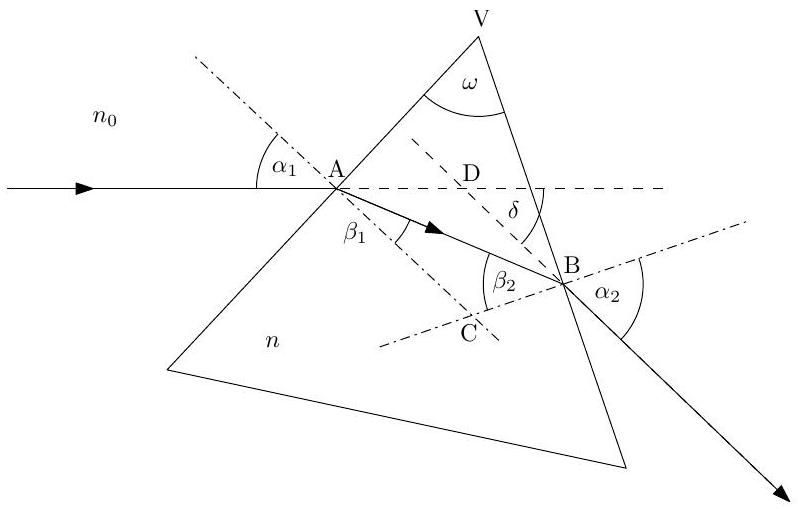
\includegraphics[max width=0.95\linewidth, center]{2024_12_03_db7ee7d12aab7219c185g-1}
	\caption{Průchod paprsku světla hranolem.}
\end{figure}


Nyní odvod’me závislost úhlové odchylky $\delta$ vystupujícího paprsku na úhlu dopadu $\alpha_{1}=\alpha$, lámavém úhlu $\omega$ a na indexu lomu skla $n$ a uvažme její průběh. Zákon lomu na prvním rozhraní je

\begin{equation}
	n_{0} \sin \alpha=n \sin \beta_{1},
\end{equation}


kde $n_{0}$ je index lomu prostředí obklopující hranol, a na druhém rozhraní

\begin{equation}
	n \sin \beta_{2}=n_{0} \sin \alpha_{2}
\end{equation}


Deviace $\delta$ je vnější úhel v trojúhelníků ABD při vrcholu D a tedy můžeme napsat


\begin{equation}
	\delta=\left(\alpha-\beta_{1}\right)+\left(\alpha_{2}-\beta_{2}\right) .
\end{equation}


Lámavý úhel $\omega$ je vnějším úhlem při vrcholu C v trojúhelníku ABC , neboť strana AC je kolmá k prvnímu rozhraní AV a strana BC je kolmá k druhému rozhraní BV, tedy:


\begin{equation}
	\omega=\beta_{1}+\beta_{2} .
\end{equation}


Deviace $\delta$ je pak podle (9.3) a (9.4) rovna

\begin{equation}
	\delta=\alpha+\alpha_{2}-\omega
\end{equation}


Vyjádříme-li $\alpha_{2}$ ze vztahů (9.1), (9.2, , 9.4 a (9.5), obdržíme závislost deviace na úhlu dopadu $\alpha$ ve tvaru

{\small \begin{equation}
	\delta=f\left(\alpha, \omega, n, n_{0}\right)=\end{equation}\\\begin{equation*}
	=\alpha-\omega+\arcsin \left[\sin \omega \sqrt{\left(\frac{n}{n_{0}}\right)^{2}-\sin ^{2} \alpha}-\cos \omega \sin \alpha\right]
	\end{equation*}
}



Tato závislost má pro realistické případy indexu lomu skla $n$ a vrcholových úhlů $\omega$ jedno minimum\\
\begin{figure}[H]
	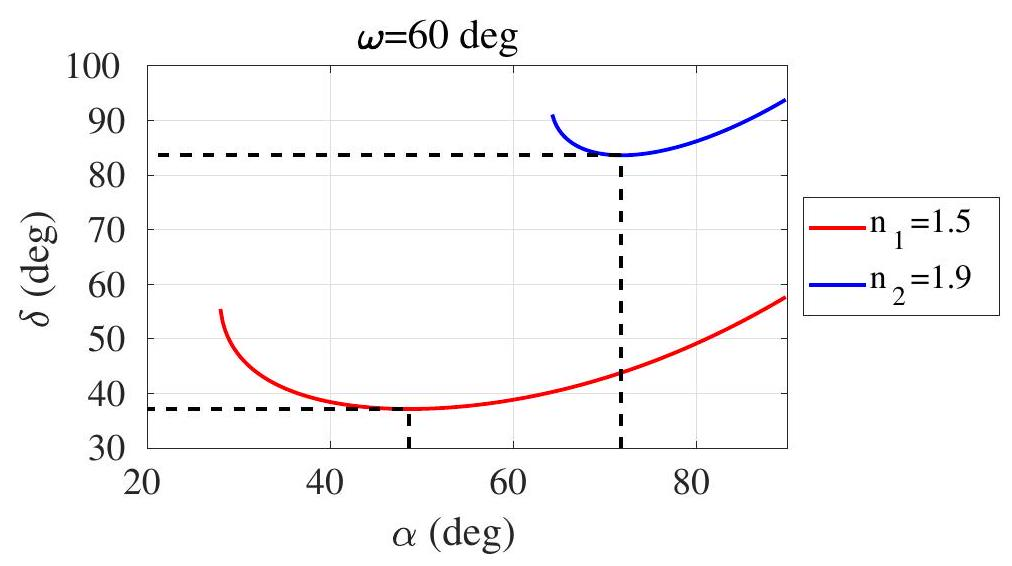
\includegraphics[max width=0.95\linewidth, center]{2024_12_03_db7ee7d12aab7219c185g-2}
	\caption{Závislost deviace paprsku na úhlu dopadu na stěnu hranolu pro indexy lomu hranolu $n_{1}=1.5$ (červená čára) a $n_{2}=1.9$ (modrá čára) vykreslená pro úhly dopadu pro něž je realizovatelný průchod paprsku přes výstupní stěnu hranolu. Závislost je vynesena pro vrcholový úhel $\omega=60^{\circ}$. Přerušované čáry vyznačují polohy příslušných minim deviace paprsku.}
\end{figure}

(viz obr. 2). Odvození podmínky pro minimum deviace z (6) je poněkud zdlouhavé. Elegantněji dojdeme k výsledku s použitím vztahu (5), jehož derivace podle $\alpha$ musí být v minimu nutně rovna 0 , tedy

\begin{equation}
	\frac{\mathrm{d} \delta}{\mathrm{~d} \alpha}=1+\frac{\mathrm{d} \alpha_{2}}{\mathrm{~d} \alpha}=0
\end{equation}


Diferencováním Snellova zákona pro první a druhou lámavou plochu, tj. rovnicí (1) resp. 2., obdržíme

\begin{equation}
	n_{0} \cos \alpha \mathrm{~d} \alpha=n \cos \beta_{1} \mathrm{~d} \beta_{1}
\end{equation}


a

\begin{equation}
	n_{0} \cos \alpha_{2} \mathrm{~d} \alpha_{2}=n \cos \beta_{2} \mathrm{~d} \beta_{2}
\end{equation}


Podělením těchto dvou rovnic a s použitím diferencované formy vztahu (4), $\mathrm{d} \beta_{1}=-\mathrm{d} \beta_{2}$, dostáváme

\begin{equation}
	\frac{\mathrm{d} \alpha_{2}}{\mathrm{~d} \alpha}=-\frac{\cos \alpha \cdot \cos \beta_{2}}{\cos \alpha_{2} \cdot \cos \beta_{1}}
\end{equation}

Po dosazení do podmínky pro minimum (7) a s využitím Snellova zákona obdržíme


\begin{equation}
	\frac{1-\sin ^{2} \alpha}{1-\sin ^{2} \alpha_{2}}=\frac{\frac{n}{n_{0}}-\sin ^{2} \alpha}{\frac{n}{n_{0}}-\sin ^{2} \alpha_{2}}
\end{equation}


Úhel dopadu $\alpha$, pro který je tato rovnost splněna tedy vede k nutné podmínce minima deviace $\delta$, $\frac{\mathrm{d} \delta}{\mathrm{d} \alpha}=0$. Protože je $\frac{n}{n_{0}}>0$, z rovnice 9 vyplývá, že úhel dopadu na hranol se rovná úhlu\\
výstupu $\alpha=\alpha_{2}$ a tedy $\beta_{1}=\beta_{2}$. To znamená, že paprsek, pro který je deviace minimální, prochází hranolem symetricky vzhledem k rovině půlící vrcholový úhel hranolu (tj. úhel $\omega$ při vrcholu V na obr. 1. Po dosazení do (5) a 4 obdržíme $\alpha=\frac{\delta_{\mathrm{m}}+\omega}{2}$ resp. $\beta_{1}=\frac{\omega}{2}$ a pod dosazení do Snellova zákona (1) pří aproximaci $n_{0} \approx 1$ pro vzduch dostáváme vztah svazující index lomu materiálu hranolu s vrcholovým úhlem a minimální deviací $\delta_{\mathrm{m}}$

\begin{equation}
	n=\frac{\sin \left(\left[\delta_{\mathrm{m}}+\omega\right] / 2\right)}{\sin (\omega / 2)} .
\end{equation}


Vrcholový úhel hranolu a minimální deviace jsou experimentálně relativně lehko méřitelné veličiny a nyní vidíme, že z nich můžeme určít i index lomu, aniž bychom potřebovali určovat navíc úhel dopadu $\alpha$.

Index lomu látek je závislý na vlnové délce světla. Tomuto jevu se říká disperze a je způsobená závislostí rychlosti šíření monochromatické elektromagnetické vlny v látce na její frekvenci. Disperze je příčinou existence tzv. rozkladu světla hranolem, o kterém se můžeme přesvědčit osvětlíme-li hranol paprskem bílého svĕtla, nebo svĕtlem z výbojky. Pozorujeme, že největší deviaci mají paprsky s barvou fialovou a nejmenší s barvou červenou. Tedy s rostoucí vlnovou délkou deviace klesá, a protože podle (10) nebo (6) většímu indexu lomu odpovídá větší deviace, klesá index lomu s rostoucí vlnovou délkou. Tato závislost se nazývá normální disperze látky a její znalost je významná z hlediska použití dané látky pro optické účely. Naším úkolem bude zjistit tuto závislost pro sklo, ze kterého je vyroben hranol, tj. určit disperzní křivku hranolu. Teoreticky disperzi můžeme popsat pomocí Cauchyho vztahu:

\begin{equation}
	n(\lambda)=A+\frac{B}{\lambda^{2}}+\frac{C}{\lambda^{4}}
\end{equation}


V aplikacích je třeba přihližet k celé řadě fyzikálních parametrů skel optických elementů (např. čoček nebo hranolů) charakterizujících jejich optické a mechanické vlastnosti. Dvěma hlavními optickými parametry uváděnými v technických specifikacích komerčně dostupných skel jsou index lomu skla $n_{\mathrm{d}}$ pro žlutou čáru d z Fraunhoferových čar a Abbeovo číslo  (viz obr. 3). Žlutá čára d o vlnové délce $\lambda_{\mathrm{d}}=587,6 \mathrm{~nm}$ je zvolena proto, že se nachází přibližně uprostřed intervalu vlnových délek viditelného spektra ( tj .380 nm až 750 nm ). Abbeovo číslo, které je převrácenou hodnotou disperzní mohutnosti skla , je definované jako

\begin{equation}
	\nu_{\mathrm{d}}=\frac{n_{\mathrm{d}}-1}{n_{\mathrm{F}}-n_{\mathrm{C}}},
\end{equation}


kde $n_{\mathrm{F}}$ a $n_{\mathrm{C}}$ jsou indexy lomu skla pro Fraunhoferovy čáry o vlnových délkách $\lambda_{F}=486,1 \mathrm{~nm}$ (modrá) resp. $\lambda_{C}=656,3 \mathrm{~nm}$ (červená). Abbeovo číslo je nepřímo úměrné rozdílu indexů lomů světla na opačných stranách viditelného spektra. Tedy, čím je Abbeovo číslo skla menší, tím více se mění index lomu s vlnovou délkou světla, a tím bude také větší chromatická vada čočky z daného skla vyrobené.

\section*{Experiment}
Pomocí goniometru změříme potřebné úhly: lámavý úhel $\omega$ hranolu a úhel $\delta_{\mathrm{m}}$ minimální deviace paprsků. Zdrojem světla bude rtuťová výbojka, která ve viditelné oblasti spektra obsahuje řadu čar o známých vlnových délkách uvedených v tabulce 1 Polohu paprsku budeme určovat vizuálně pomocí nitkového kříže umístěného v ohniskové rovině okuláru dalekohledu, do kterého zobrazíme vstupní štěrbinu kolimátoru osvětlenou výbojkou při měření úhlu minimální deviace.

Vlastní měření se provádí na goniometru SG-5, který má pevné rameno s kolimátorem a otočný stolek s měřeným hranolem. Polohu stolku a dalekohledu lze velmi přesně nastavit hrubým a jemným posuvem a číst ji s přesností jednotek úhlových vteřin. Způsob manipulace a odečítání úhlů na stupnici je popsáno v návodu na obsluhu tohoto goniometru. Před měřením je třeba provést justování hranolu, které spočívá v nastavení lámavých ploch kolmo na optickou osu dalekohledu.\\
\begin{figure}[H]
	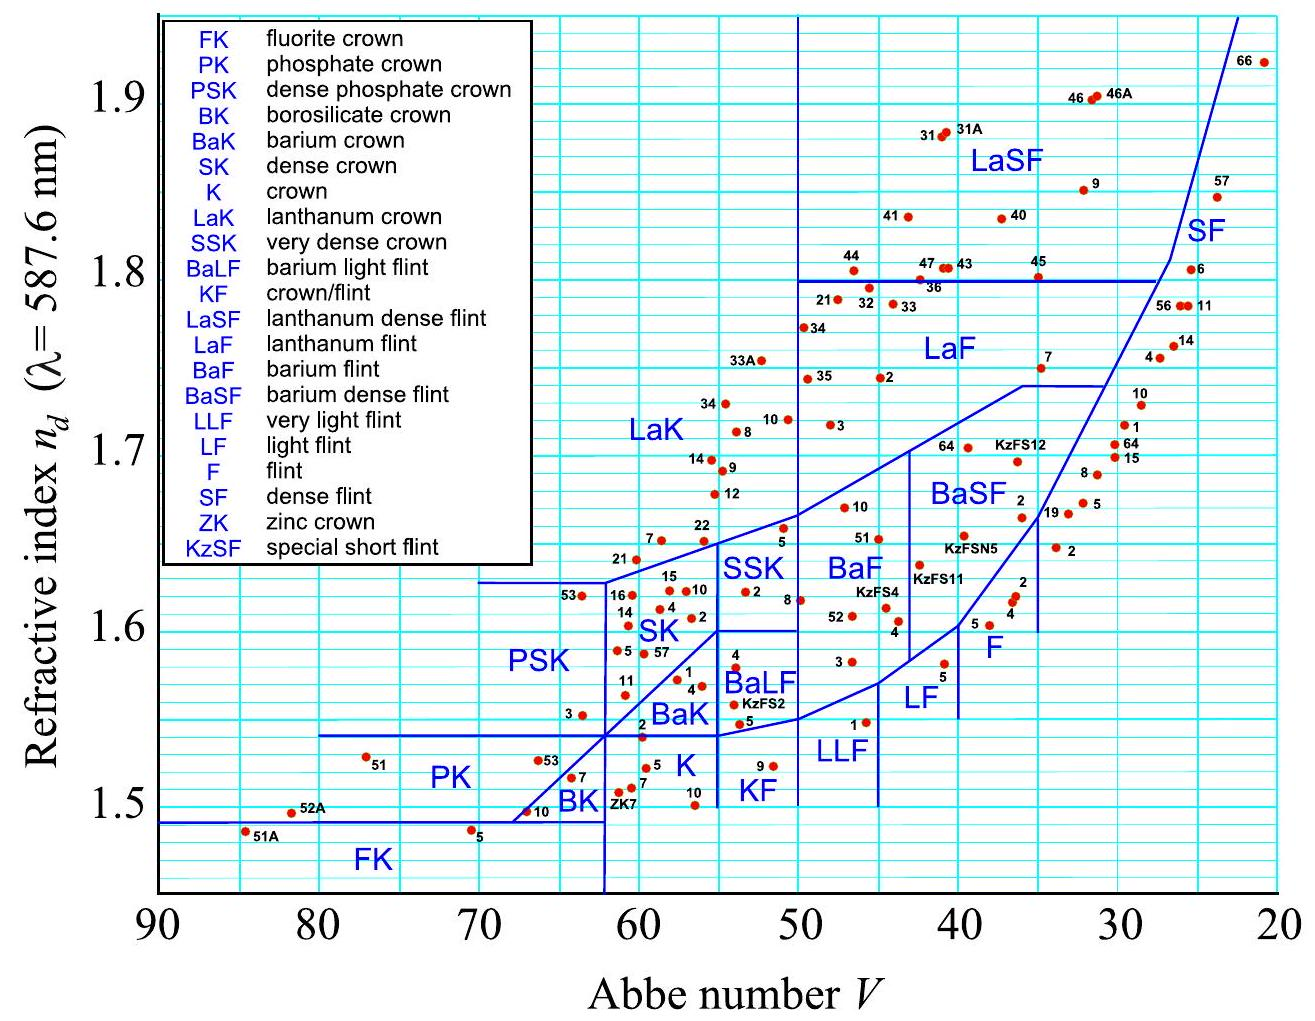
\includegraphics[max width=0.95\linewidth, center]{2024_12_03_db7ee7d12aab7219c185g-4(1)}
	\caption{Abbeův diagram zobrazující Abbeovo číslo (zde $V$ ) oproti indexu lomu žluté spektrální čáry $n_{\mathrm{d}}$ pro sérii různých typů skel (číslované tečky). Skla jsou klasifikována podle Schottova kódu, který odráží jejich složení (písmenná část kódu) a polohu v diagramu (číselná část kódu)}
\end{figure}
 

Provádí se nakláněním stolečku regulačními šrouby. Kolmost se kontroluje autokolimační metodou: nitkový kříž osvětlený žárovkou v okuláru se po odrazu od justované lámavé plochy hranolu zobrazí zpět do ohniskové roviny okuláru dalekohledu. Při ztotožnění nitkového kříže se svým obrazem je lámavá plocha kolmá k optické ose dalekohledu. Postup opakujeme několikrát.

Měření lámavého úhlu $\omega$ hranolu provádíme tak, že změříme úhel, který spolu svírají paprsky kolmé k lámavým plochám. Je-li úhel mezi kolmicemi $\psi_{1}-\psi_{2}$, je lámavý úhel

\begin{equation}
	\omega=180-\left(\psi_{1}-\psi_{2}\right)
\end{equation}


Úhlové polohy dalekohledu $\psi_{1}$ a $\psi_{2}$, kdy je optická osa dalekohledu kolmá na první resp. druhou lámavou plochu hranolu, nastavíme užitím autokolimační metody. Úhly $\psi_{1}$ a $\psi_{2}$ pak odečítáme na stupnici spojené s jednou z os rotace stolečku pozorované přes mikroskop umístěný na spodní části dalekohledu. Při měření otáčíme dalekohledem z polohy $\psi_{1}$ do polohy $\psi_{2}$, aniž bychom otáčeli stolečkem s hranolem (viz obr. 5). Pro zvýšení přesnosti určení $\omega$ a určení nejistoty provádíme měření několika dvojic úhlů $\psi_{1}, \psi_{2}$.

Měření úhlu minimální deviace $\delta_{\mathrm{m}}$ provádíme pro každou spektrální čáru rtuti v bodě obratu paprsku. Minimální deviaci najdeme tak, že měníme úhel dopadu světla z výbojky na hranol otá-\\

\begin{figure}[H]
	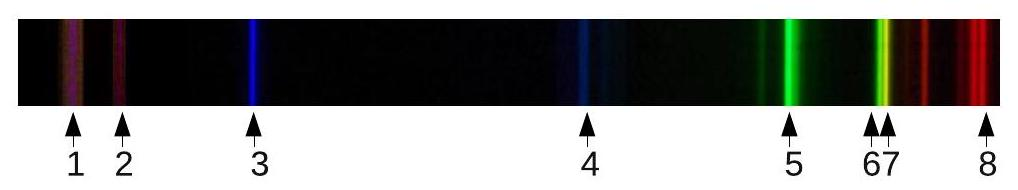
\includegraphics[max width=0.95\linewidth, center]{2024_12_03_db7ee7d12aab7219c185g-4}
	\caption{Upravená fotografie spektra rtutové výbojky. Očíslovány jsou čáry, jejichž vlnové délky jsou uvedeny v tabulce 1.}
\end{figure}



Tabulka 1: Vlnové délky vybraných čar spektra rtutové výbojky.

\begin{center}
	\begin{tabular}{|c|l|l|l|}
		\hline
		$\lambda$ (nm) & barva & poznámka & n\\
		\hline
		404,7 & fialová & silnější & 1 \\
		407,8 & fialová & slabší & 2 \\
		435,8 & modrá & silná & 3 \\
		491,6 & modrozelená & jasná & 4 \\
		546,1 & zelená & silná & 5 \\
		576,9 & žlutá & silná & 6 \\
		579,1 & žlutá & silná & 7 \\
		585,9 & oranžová & slabá &  \\
		607,3 & červená & slabá &  \\
		623,4 & červená & silná & 8 \\
		690,7 & červená & slabá &  \\
		\hline
	\end{tabular}
\end{center}


\begin{figure}[H]
		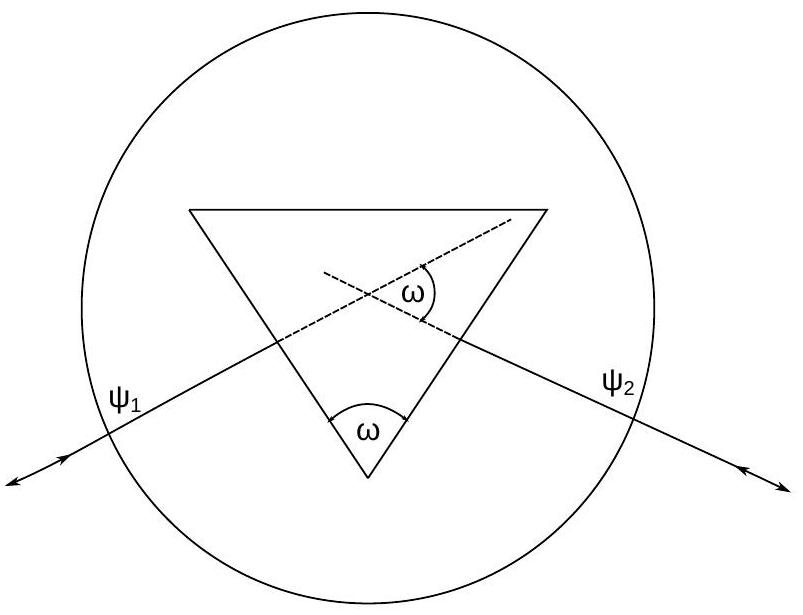
\includegraphics[max width=0.95\linewidth, center]{2024_12_03_db7ee7d12aab7219c185g-5}
		\caption{Měření lámavého úhlu hranolu.}
\end{figure}


čením stolečku s hranolem a pozorujeme pohyb dané spektrální čáry. Zatímco stolečkem otáčíme stále v určitém zvoleném směru, směr pohybu spektrální čáry vystupující z hranolu se v bodě minimální deviace obrátí (tj. deviace se nejdříve zmenšuje a pak zvětšuje). Bod obratu pohybu spektrální čáry nejlépe přibližně nalezneme prostým okem a až poté zpřesníme určení jeho polohy při pozorování dalekohledem. Nicméně, nemůžeme změřit úhlovou polohu paprsku vstupujícího do hranolu (museli bychom sejmout hranol), a tedy nelze určit minimální deviaci z rozdílu úhlu mezi vstupujícím a vystupujícím paprskem. Proto postupujeme tak, že změříme úhlovou polohu $\phi_{1}$ vystupujícího paprsku v bodě minimální deviace při jeho vstupu do hranolu první lámavou plochou, pak otočíme stolek s hranolem tak, aby paprsek vstupoval do hranolu druhou lámavou plochou a změříme polohu vystupujícího paprsku $\phi_{2} \mathrm{v}$ bodě minimální deviace při obráceném směru průchodu paprsku hranolem (viz obr. 6). Stolkem s hranolem přitom otáćíme v ose, která není spojená s rotací úhlové stupnice, abychom mohli určit rozdíl úhlů. Rozdíl těchto úhlů je dvojnásobek minimální deviace:

\begin{equation}
	\delta_{\mathrm{m}}=\left(\phi_{1}-\phi_{2}\right) / 2
\end{equation}


Při měření postupujeme tak, že nejdříve změříme pro všechny zvolené spektrální čáry polohy $\phi_{1}$, pak hranol otočíme a měříme polohy $\phi_{2}$ u stejných spektrálních čar.

Index lomu pro každou spektrální čáru vypočítáme ze vztahu 10. Příslušnou vlnovou délku najdeme v tabulce 1 nebo přímo v tabulkách.\\
\begin{figure}
	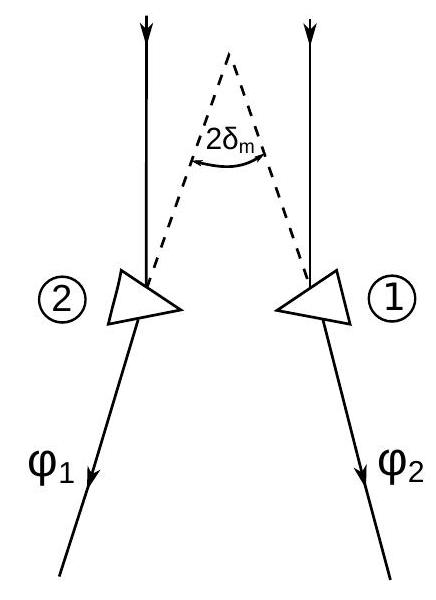
\includegraphics[max width=0.45\linewidth, center]{2024_12_03_db7ee7d12aab7219c185g-6}
	\caption{Měření úhlu minimální deviace z rozdíl úhlů $\phi_{1}$ a $\phi_{2}$, pod kterými pozorujeme paprsky vystupující z hranolu při vstupu přes první resp. druhou lámavou stěnu (poloha hranolu 1 resp. 2).}
\end{figure}


	
		\section{Měření}
		Lámavý úhel měříme vícekrát, přičemž stolek s hranolem vždy otočíme. Používáme formuli (15). Získáváme:\\
		\begin{center}
			\begin{tabular}{rr|r}

			 $\psi_{1}$[°] & $\psi_{2}$ [°] & $\omega$[°] \\

			 286.315 & 146.078 & 39.763 \\
			 276.671 & 136.443 & 39.772 \\
			 270.613 & 130.383 & 39.770 \\
			 275.418 & 135.195 & 39.777 \\
			 279.265 & 139.030 & 39.765 \\

		\end{tabular}
		\end{center}
		\begin{equation}
			\omega = 39.769 \pm 0.003 \,\mathrm{^\circ} = 39^\circ 46'8.4'' \pm 10.8"
		\end{equation}
		Následně využijeme rtuťové výbojky a měříme úhly dopadu různých spektrálních čar, resp. vlnových délek. Toto provedeme nejdříve pro jednu polohu hranolu (tak, jak je zmíněno v úvodu), a poté pro polohu druhou.
		Získáváme:\\ \\
		\begin{tabular}{llll}
			$\lambda \,\mathrm{[nm]} $ & Barva       & $\phi_1 \,\mathrm{[^\circ]}$        &  $\phi_2 \,\mathrm{[^\circ]}$           \\ \hline
			623.4      & Cervena     & 184.020833 & 228.609722 \\
			576.9      & Zluta       & 183.960833 & 228.684167 \\
			491.6      & Modrozelena & 183.738056 & 228.901111 \\
			435.8      & Modra       & 183.523611 & 229.107778 \\
			404.6      & Fialova     & 183.362778 & 229.266944
		\end{tabular}\\
		Z toho získáme úhel minimální deviace, a tím i index lomu materiálu $n$:
		
		\begin{tabular}{ll|ll}
			$\lambda \,\mathrm{[nm]}$ & Barva       & $\delta\,\mathrm{[^\circ]}$     & n                 \\
			623.4        & Cervena     & 22.294 & 1.5157+/-0.00009 \\
			576.9        & Zluta       & 22.362 & 1.5171+/-0.00009 \\
			491.6        & Modroz. & 22.582 & 1.5220+/-0.00009 \\
			435.8        & Modra       & 22.792 & 1.5266+/-0.00009 \\
			404.6        & Fialova     & 22.952 & 1.5301+/-0.00009
		\end{tabular}
		
		
		
		následně hodnoty indexu lomu vykreslíme v závislosti na vlnové délce a proložíme Cauchyho vztahem:
		
		\begin{figure}[H]
			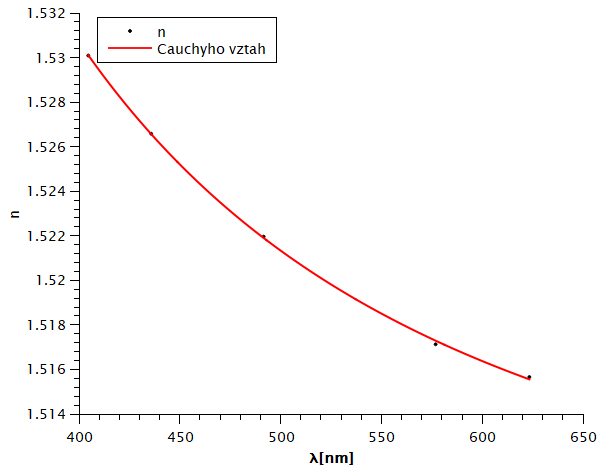
\includegraphics[width=0.95\linewidth,center]{fit}
		\end{figure}
		Z čehož získáváme hodnoty konstant
		\begin{gather*}
			A = 1.50493 \pm 0.00019 \\
			B = 4.11 \pm 0.04 \,.10^3 \,\mathrm{nm^2}
		\end{gather*}
		Pro Abbeovo číslo získáváme hodnotu:
		\begin{equation*}
			\nu_d = 65.8 \pm 0.7
		\end{equation*}
		Použili jsme Hranol 3 z optického skla H-K9L, pro nějž dle tabulek Abbeovo číslo nabývá hodnoty $\nu _d = 64.90$ Pozorujeme tedy, že od skutečných hodnot nejsme příliš daleko.
		
		\section{Závěr}
		Podařilo se nám splnit veškeré zadané úkoly a získat hodnoty hledaných veličin. Finální hodnota - Abbeovo číslo - se od udané hodnoty liší velmi málo.
		
	
		

		
		
		
		
		
		% Nakonec nezapomeňte projet text programem vlna nebo vlnka, např.
		% 	vlna -m -l -n mojeuloha.tex
		% nebo zkontrolovat a opravit jednopísmenné předložky na koncích řádků ručně.
	\end{multicols}
\end{document}
